%%%%%%%%%%%%%%%%%%%%%%%%%%%%%%%%%%%%%%%%%
% Masters/Doctoral Thesis 
% LaTeX Template
% Version 2.4 (22/11/16)
%
% This template has been downloaded from:
% http://www.LaTeXTemplates.com
%
% Version 2.x major modifications by:
% Vel (vel@latextemplates.com)
%
% This template is based on a template by:
% Steve Gunn (http://users.ecs.soton.ac.uk/srg/softwaretools/document/templates/)
% Sunil Patel (http://www.sunilpatel.co.uk/thesis-template/)
%
% Template license:
% CC BY-NC-SA 3.0 (http://creativecommons.org/licenses/by-nc-sa/3.0/)
%
%%%%%%%%%%%%%%%%%%%%%%%%%%%%%%%%%%%%%%%%%

%----------------------------------------------------------------------------------------
%	PACKAGES AND OTHER DOCUMENT CONFIGURATIONS
%----------------------------------------------------------------------------------------

\documentclass[
11pt, % The default document font size, options: 10pt, 11pt, 12pt
%oneside, % Two side (alternating margins) for binding by default, uncomment to switch to one side
english, % ngerman for German
singlespacing, % Single line spacing, alternatives: onehalfspacing or doublespacing
%draft, % Uncomment to enable draft mode (no pictures, no links, overfull hboxes indicated)
%nolistspacing, % If the document is onehalfspacing or doublespacing, uncomment this to set spacing in lists to single
%liststotoc, % Uncomment to add the list of figures/tables/etc to the table of contents
%toctotoc, % Uncomment to add the main table of contents to the table of contents
%parskip, % Uncomment to add space between paragraphs
%nohyperref, % Uncomment to not load the hyperref package
headsepline, % Uncomment to get a line under the header
%chapterinoneline, % Uncomment to place the chapter title next to the number on one line
%consistentlayout, % Uncomment to change the layout of the declaration, abstract and acknowledgements pages to match the default layout
]{MastersDoctoralThesis} % The class file specifying the document structure

\usepackage[utf8]{inputenc} % Required for inputting international characters
\usepackage[T1]{fontenc} % Output font encoding for international characters

\usepackage{palatino} % Use the Palatino font by default

\usepackage[backend=bibtex,style=numeric,natbib=true]{biblatex} % Use the bibtex backend with the authoryear citation style (which resembles APA)

\addbibresource{bibliography.bib} % The filename of the bibliography

\usepackage[autostyle=true]{csquotes} % Required to generate language-dependent quotes in the bibliography

%----------------------------------------------------------------------------------------
%	MARGIN SETTINGS
%----------------------------------------------------------------------------------------

\geometry{
	paper=a4paper, % Change to letterpaper for US letter
	inner=2.5cm, % Inner margin
	outer=3.8cm, % Outer margin
	bindingoffset=.5cm, % Binding offset
	top=1.5cm, % Top margin
	bottom=1.5cm, % Bottom margin
	%showframe, % Uncomment to show how the type block is set on the page
}

%----------------------------------------------------------------------------------------
%	THESIS INFORMATION
%----------------------------------------------------------------------------------------

\thesistitle{Modeling Temporal point processes using Recurrent Neural Nets} % Your thesis title, this is used in the title and abstract, print it elsewhere with \ttitle
\supervisor{Dr. Mark \textsc{Herbster}} % Your supervisor's name, this is used in the title page, print it elsewhere with \supname
\examiner{} % Your examiner's name, this is not currently used anywhere in the template, print it elsewhere with \examname
\degree{Master of Science} % Your degree name, this is used in the title page and abstract, print it elsewhere with \degreename
\author{Badrul \textsc{Alom}} % Your name, this is used in the title page and abstract, print it elsewhere with \authorname
\addresses{} % Your address, this is not currently used anywhere in the template, print it elsewhere with \addressname

\subject{Data Science} % Your subject area, this is not currently used anywhere in the template, print it elsewhere with \subjectname
\keywords{} % Keywords for your thesis, this is not currently used anywhere in the template, print it elsewhere with \keywordnames
\university{\href{http://www.ucl.ac.uk}{University College London}} % Your university's name and URL, this is used in the title page and abstract, print it elsewhere with \univname
\department{Department of Computer Science} % Your department's name and URL, this is used in the title page and abstract, print it elsewhere with \deptname
\group{\href{http://researchgroup.university.com}{Research Group Name}} % Your research group's name and URL, this is used in the title page, print it elsewhere with \groupname
\faculty{\href{http://faculty.university.com}{Faculty Name}} % Your faculty's name and URL, this is used in the title page and abstract, print it elsewhere with \facname

\AtBeginDocument{
\hypersetup{pdftitle=\ttitle} % Set the PDF's title to your title
\hypersetup{pdfauthor=\authorname} % Set the PDF's author to your name
\hypersetup{pdfkeywords=\keywordnames} % Set the PDF's keywords to your keywords
}

\begin{document}

\frontmatter % Use roman page numbering style (i, ii, iii, iv...) for the pre-content pages

\pagestyle{plain} % Default to the plain heading style until the thesis style is called for the body content

%----------------------------------------------------------------------------------------
%	TITLE PAGE
%----------------------------------------------------------------------------------------

\begin{titlepage}
\begin{center}

\vspace*{.06\textheight}
{\scshape\LARGE \univname\par}\vspace{1.5cm} % University name
\textsc{\Large Doctoral Thesis}\\[0.5cm] % Thesis type

\HRule \\[0.4cm] % Horizontal line
{\huge \bfseries \ttitle\par}\vspace{0.4cm} % Thesis title
\HRule \\[1.5cm] % Horizontal line
 
\begin{minipage}[t]{0.4\textwidth}
\begin{flushleft} \large
\emph{Author:}\\
\href{http://www.johnsmith.com}{\authorname} % Author name - remove the \href bracket to remove the link
\end{flushleft}
\end{minipage}
\begin{minipage}[t]{0.4\textwidth}
\begin{flushright} \large
\emph{Supervisor:} \\
{\supname} % Supervisor name - remove the \href bracket to remove the link  
\\
\emph{Advised by:} \\
{Pedro Mediano (Emotech Ltd.)} 
\end{flushright}
\end{minipage}\\[3cm]
 
\vfill

\large \textit{A thesis submitted in fulfillment of the requirements\\ for the degree of \degreename}\\[0.3cm] % University requirement text
\textit{in the}\\[0.4cm]
\deptname\\[2cm] % Research group name and department name
 
\vfill

{\large \today}\\[4cm] % Date
%\includegraphics{Logo} % University/department logo - uncomment to place it
 
\vfill
\end{center}
\end{titlepage}

%----------------------------------------------------------------------------------------
%	DECLARATION PAGE
%----------------------------------------------------------------------------------------

\begin{declaration}
\addchaptertocentry{\authorshipname} % Add the declaration to the table of contents
\noindent I, \authorname, declare that this thesis titled, \enquote{\ttitle} and the work presented in it are my own. I confirm that:

\begin{itemize} 
\item This work was done wholly or mainly while in candidature for a research degree at this University.
\item Where any part of this thesis has previously been submitted for a degree or any other qualification at this University or any other institution, this has been clearly stated.
\item Where I have consulted the published work of others, this is always clearly attributed.
\item Where I have quoted from the work of others, the source is always given. With the exception of such quotations, this thesis is entirely my own work.
\item I have acknowledged all main sources of help.
\item Where the thesis is based on work done by myself jointly with others, I have made clear exactly what was done by others and what I have contributed myself.\\
\end{itemize}
 
\noindent Signed:\\
\rule[0.5em]{25em}{0.5pt} % This prints a line for the signature
 
\noindent Date:\\
\rule[0.5em]{25em}{0.5pt} % This prints a line to write the date
\end{declaration}


%----------------------------------------------------------------------------------------
%	ABSTRACT PAGE
%----------------------------------------------------------------------------------------

\begin{abstract}
\addchaptertocentry{\abstractname} % Add the abstract to the table of contents
tbc
\end{abstract}


%----------------------------------------------------------------------------------------
%	THESIS CONTENT - CHAPTERS
%----------------------------------------------------------------------------------------

\mainmatter % Begin numeric (1,2,3...) page numbering

\pagestyle{thesis} % Return the page headers back to the "thesis" style

% Include the chapters of the thesis as separate files from the Chapters folder
% Uncomment the lines as you write the chapters

% Chapter 1

\chapter{Introduction} % Introduction

\label{Chapter1} % For referencing the chapter elsewhere, use \ref{Chapter1} 

%----------------------------------------------------------------------------------------

% Define some commands to keep the formatting separated from the content 
\newcommand{\keyword}[1]{\textbf{#1}}
\newcommand{\tabhead}[1]{\textbf{#1}}
\newcommand{\code}[1]{\texttt{#1}}
\newcommand{\file}[1]{\texttt{\bfseries#1}}
\newcommand{\option}[1]{\texttt{\itshape#1}}

%----------------------------------------------------------------------------------------

The modeling of event sequences is useful across industries. For instance the periods in which a customer makes an online purchase can help determine the optimal periods for target marketing. The times at which public transport users tend to travel can help better manage resources to meet demand. The times at which a medical illness re-occurs can help predict future episodes.
 
In all these cases modeling the temporal behaviour of the system is important in predicting the next event. At an aggregate level, behaviour may appear to be deterministic, such as the times at which peak rush-hour occurs, but such behaviour is often composed of thousands or millions of individual stochastic processes such as the decisions made by individuals as to whether to leave work at 5pm or continue working a little longer.

While the modeling of aggregate patterns is well understood, these models ofen breakdown when applied to customizing results for individual users. At this level the temporal patterns of an individual combined with the behaviour of the population may be a better preditor of event timing. For instance, sticking with the example above, the times at which a person has lunch during the day may help predict that they will finish work a little later.

while the area of product recommendation has received extensive attention in recent years, the area of recommendation timing less so. This research looks at how we can model the temporal behaviour of individuals, and whether deep learning is better able to learn these patterns than other methods.

\section{Motivation}

We take as our context for this research, the goal of estimating the probability that a user of a home-audio device would like to listen to music right now, based on their listening-event history. 

The raw data is a series of timestamps denoting when songs were played. The implicit assumption is that a persons playlist history contains a temporal pattern such as a combination of daily and weekly schedule, that can be modelled. This concept can also be applied to other areas where a temporal pattern is thought to exist at an individual user level, such as the repeat purchase of household products, or the sleeping and eating habits of a person.

The objective of the research is to evaluate the effectiveness of several different techniques for determining the probability of a user listening to music in a given period. One such application of this would be home audio devices which could anticipate when a user would like to listen to music and play without user intervention.

The research was guided by Emotech Ltd. the creators of Olly \parencite{Olly}.

\section{Point Processes}

One way of modeling the problem is as series of events and non-events known as a temporal point process. This has a rich history of methods as outlined in the literature review. 


\section{The dataset}
The dataset being used in this analysis is the LastFM1k dataset containing the listening history of a thousand LastFM listeners.

The dataset contains the timestamp, userId, and trackId of users listening habits over a number of years (2005-2009).

\section{Structure of the report}
tbc

% Chapter 2

\chapter{Literature Review} % Introduction

\label{Chapter2} % 

Event prediction is alternatively referred to in literature as sequence predictions and temporal point processes. The problem can be defined mathematically as determining:

$$p(x_t | x_h)  $$
where h is the event history sequence, ${t-n ... t-1}$.

\section{Point Processes}

This is one of the most widely used method for modeling event sequences. A temporal point process \parencite{DaleyJones} is a way of modeling events data with $t$ being a sequence of a fixed period interval with $t_i \epsilon R + and i \epsilon Z+$. 

It can be modelled as a series of inter-event times (time until next event) or the number of events occurring in the interval. Examples of point processes are the times between financial transactions \parencite{EngleRusell}, and the times at which a customer makes a purchase from an online retailer *** insert ref***.

At its simplest a point process can be represented as:
$${\xi =\sum _{i=1}^{n}\delta _{X_{i}},}$$

where $\delta$ denotes the Dirac measure, a probability measure of whether a set contains point x or not.

Point processe models seek to estimate the probability of an event happening at time t, based on an event history upto, but not including, time $t$. 

There are different ways of representing point process data as shown in figure \ref{fig:fig1}, with the inter-event time being the most common. 

\begin{figure}[h!]
	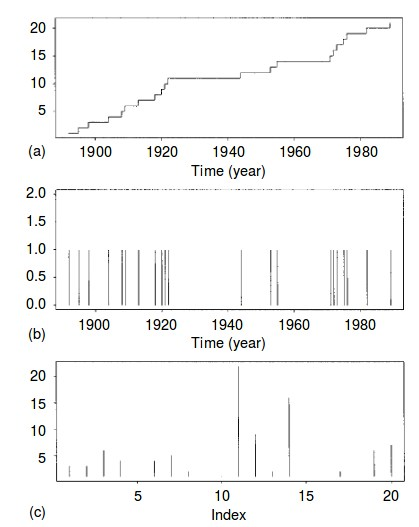
\includegraphics[width=7cm, keepaspectratio]{fig001.jpg}
	\caption{Three different representations of the same point-process a) cumulative count b) date of occurence c) interval time between floods}
	\label{fig:fig1}
\end{figure}

\subsection{Time-series analysis}


\subsection{Conditional Intensity Function}

A conditional intensity function is the key part of modeling point processes \parencite{DuWang}. In this method the probability of an event $\lambda(t)$ is derived from a stochastic model such as the Poisson process. 

Conditional intensity functions can be inhomogenous such as with a Gaussian Kernel $\lambda(t) = \sum^k_{i=1}\alpha(2\pi \sigma^2_i)^{-1/2}exp(-(t-c_i)^2/\sigma^2_i)$
, for $t \epsilon [0,T]$ where $c_i$ and $\sigma$ are fixed center and standard deviations, respectively, and $\alpha_i$ is the weight for kernel i.

Or they can vary in intensity, such as with the self-exciting (Hawkes) process where the intensity is determined by previous events through the parametric form $\lambda(t) = \mu + \beta \sum_{t_i<t}g(t-t_i) where g is some non-negative kernel function.$

As noted by Wass et. al \parencite{Wass}, conventional point process models often make unrealistic assumptions about the generative processes of the event sequences. The conditional intensity function make various parametric assumptions about the latent dynamics governing the generation of the observed point patterns. As a consequence, model misspecification can cause significantly degraded
performance using point process models.

\section{Deep RNN Point Process Models}

In recent years deep learning has demonstrated the power to learn hierarchical nonlinear patterns on large-scale datasets \parencite{DL} through multiple layers of abstraction (e.g. multi-layer feedforward neural networks). It has achieved state-of-the-art performances on a wide range of applications, such as computer vision \parencite{ImageNet}, natural language processing \parencite{Socher}, and protein structure prediction \parencite{Lena}.

However it has not been applied to temporal point processes until recently with Xiao et. al \parencite{Wass} applying Generative Adversarial Networks (GANS) to the problem. GANs consist of two neural network models - a generator tasked with generating (i.e. predicting) a future sequence of events based on the history, and a discriminator tasked with detecting the true (fround truth) sequence amongst the generated ones.

For measuring the loss between a generated and true sequence, the authors found the Wassertein-Distance \parencite{WassGAN} performed better than Maximum Likihood Estimate (MLE) which they remarked "may suffer from mode dropping or get stuck in an inferior local minimum".

Their findings showed that where as parametric point process models work better with problems where a parametetric form exists, with real world data a GAN model with Wasserterin-Distance outperformed all other models (including an RNN model using MLE). This signals a promising new direction for temporal point process research.

 
% Chapter 3

\chapter{Methodology} % Methodology

\label{Chapter3} % For referencing the chapter elsewhere, use \ref{Chapter3} 

The research set out to evaluate different methods for estimating when a listening event is likely to occur. These were:

* Bayesian Counting
* Logistic Regression
* SVM
* Gaussian Processes
* Recurrent Neural Networks

The methodology employed is typical of that within the data science community, and as seen in online Kaggle competitions. Namely to start with preliminary analysis that will help understand the data better, then devise a test and training datasets that can be used across multiple models, with the main performance criteria being on how well the models perform on test data.

Python, via Jupyter notebooks was the primary source of analysis with some SQL as the data was manipualated and stored in a SqlLite3 database first.

Note: In the interest of time, analysis was carried out on 381 of the full 1000 user dataset.

\section{Preliminary analysis}

\subsection{Context}

Let us first consider the real-world aspect of the data we have - the timestamps on which users played a song. This does not necessarily mean they played the song in its entirety. Indeed initial analysis shows plenty of cases where a song was started, seconds after the previous one, suggesting that the dataset contains both tracks that were played and tracks that were skipped. For our purposes we can consider both these to be the same as they both indicate that the user was interested in playing music at time $t$.

We can also assume that the song plays are not i.i.d, in that the probability of a play event at time t+1 is significantly higher if there was an event at time t. 

\subsection{Basic statistics} 

We start with some basic information about the raw data file that was recieved. 
Num. of rows: 7,500,000
Num. of users: 381
Num. of unique timestamps: 7,226,934
earliest timestamp: 2005-02-14 00:02:10
latest timestamp: 2009-06-19 17:37:23

What does this tell us? Well we can deduce there are approximately 19.6k timestamps per user on average. This feels like a high number. Fig \ref{fig:fig1}

\begin{figure}[h!]
	\centering
	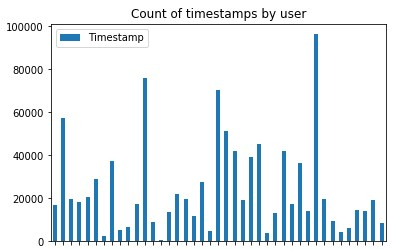
\includegraphics[width=7cm, keepaspectratio,]{fig002.jpg}
	\caption{}
	\label{fig:fig2}
\end{figure} 


\subsection{Outlier analysis} 


\section{Bayesian Inference}

Here we apply a counting process


\section{How to cite references in Latex}
\parencite{Reference1}

\medskip

This document is an example of \texttt{thebibliography} environment using 
in bibliography management. Three items are cited: \textit{The \LaTeX\ Companion} 
book \cite{latexcompanion}, the Einstein journal paper \cite{einstein}, and the 
Donald Knuth's website \cite{knuthwebsite}. The \LaTeX\ related items are
\cite{latexcompanion,knuthwebsite}. 

\medskip

%% Chapter 5

\chapter{Evaluation} % Methodology

\label{Chapter5} % For referencing the chapter elsewhere, use \ref{Chapter5} 

In this chapter we present the results of the evaluation starting with the best result obtained from each model from different hyper-parameter testing.

The performance of each model is then discussed further in the sections that follow. 

\section{Results summary}

Within the context of a home audio decide, the cost of mistakenly suggesting a user wants to listen to music is higher than the cost of not suggesting at all. We therefore focus our results on the predictions where a 'play' event was predicted by the model and examine both the precision and recall scores for both the hidden periods for existing users as well as new users.

All models required a number of runs to try and determine the best hyper-parameters, as dicusssed in the next few chapters, and it may be the case that hyper-parameter settings exist for each model that would provide a boost in performance.

Looking at the F1-score we see that the RNN model performed the best overall with the logistic regression model close behind. Looking solely at new users we can say that the RNN model makes correct guesses 72\% of the time, and being well balanced between being right its guesses (precision), and guessing all of the time right events (recall). 

We see a somewhat stronger performance on recall, relative to logistic regression on the hidden periods assessment. This can be considered the performance under a 'busuines-as-usual' scenario beyond the cold-start phase. 

However as discussed in the RNN results section, the results are not as clear cut when we try to separate out the feature engineering element of our model from the LSTM specific element. Recall that our dataset consisted of rows of data, each one containing information from time-lags t-1, t-2 etc.

In theory an LSTM ought to be able to learn such features by itself based on its architecture. As part of the testing it was found that RNN recall reduces from 72\% to around 3\% when time lags 1-5 are not directly encoded. This indicates a clear failure to pick up the most important of time-lags t-1. Speculation as to why is discussed in more detail in the RNN results section.

\section{Adaptability to new users}

\begin{figure}[h!]
	\centering
	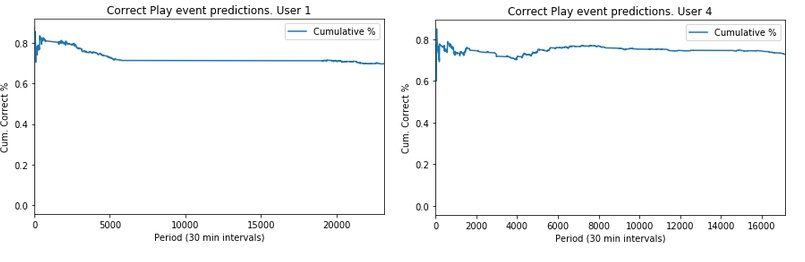
\includegraphics[width=7cm, keepaspectratio,]{fig008a.jpg}
	\caption{}
	\label{fig:fig8a}
\end{figure} 

\begin{figure}[h!]
	\centering
	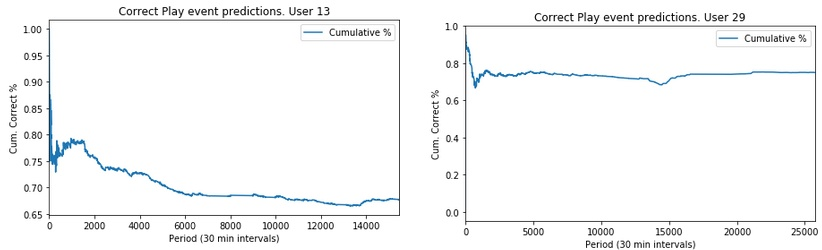
\includegraphics[width=7cm, keepaspectratio,]{fig008b.jpg}
	\caption{}
	\label{fig:fig8b}
\end{figure} 

\begin{figure}[h!]
	\centering
	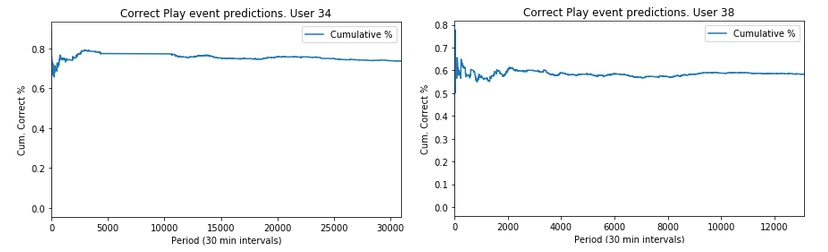
\includegraphics[width=7cm, keepaspectratio,]{fig008c.jpg}
	\caption{}
	\label{fig:fig8c}
\end{figure} 

\begin{figure}[h!]
	\centering
	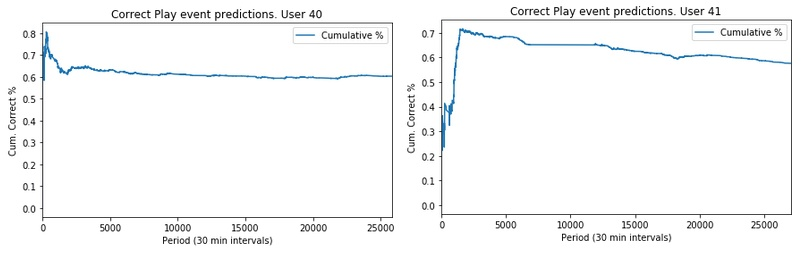
\includegraphics[width=7cm, keepaspectratio,]{fig008d.jpg}
	\caption{}
	\label{fig:fig8d}
\end{figure} 

\begin{figure}[h!]
	\centering
	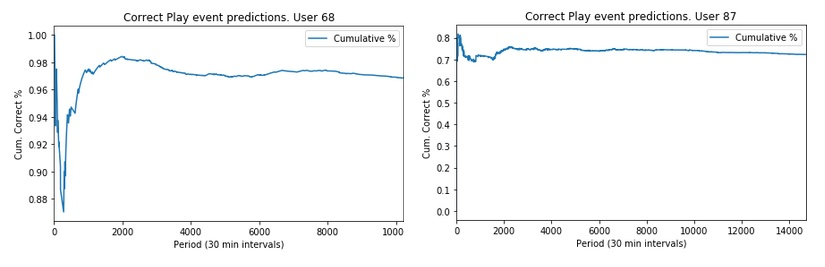
\includegraphics[width=7cm, keepaspectratio,]{fig008e.jpg}
	\caption{}
	\label{fig:fig8e}
\end{figure} 

\section{Beta-Binomial model}

\section{Logistic Regression}

\section{RNN}

 
% Chapter Template

\chapter{Summary} % Main chapter title

\label{ChapterX} % Change X to a consecutive number; for referencing this chapter elsewhere, use \ref{ChapterX}


\section{Conclusion}


 
%----------------------------------------------------------------------------------------
%	THESIS CONTENT - APPENDICES
%----------------------------------------------------------------------------------------

\appendix % Cue to tell LaTeX that the following "chapters" are Appendices

% Include the appendices of the thesis as separate files from the Appendices folder
% Uncomment the lines as you write the Appendices

% Appendix A

\chapter{Appendices}

\section{A. Further detail of experiments}

\section{Bayesian Inference}

Prior probabilities were calculated or each half-hourly period in a week. Fig \ref{fig10b} shows the calculations for the first 2.5 hours of a Sunday (d-hour-hh format). 

Our parameter of interest is the mean for the Beta distribution representing the probability of play in that time period. We estimate this by calculating probability of a play (total plays in period / count of plays and non-plays) per user, then taking the mean and variance across users. $a$ and $b$ are then determined as:
$a = (\frac{(1- \mu)}{\sigma} - \frac{1}{\mu}) \mu^2$
and
$\beta=\alpha\left(\frac{1}{\mu}-1\right)$.

\begin{figure}[h!]
	\centering
	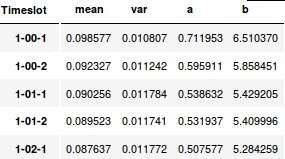
\includegraphics[width=4cm, keepaspectratio,]{fig010b.jpg}
	\caption{}
	\label{fig10b}
\end{figure} 

This allows us to visualize the prior probability for any given time period as shown in \ref{fig10c}.

\begin{figure}[h!]
	\centering
	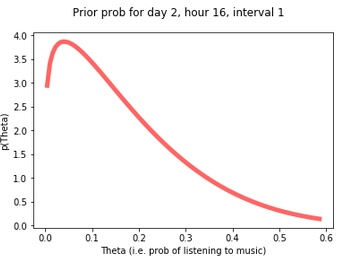
\includegraphics[width=5cm, keepaspectratio,]{fig010c.jpg}
	\caption{}
	\label{fig10c}
\end{figure} 

Once established we can calculate the liklihood of an individual user listening to music in a given time period by passing their observations as they come in for a specific timeslot $s$: $(H_{t,s})$ , into a Beta-Binomial formula to determine the probability of listening at the next occurence of that time slot as shown in <TBC>

Finally the threshold at which we determine that a probability constitutes a Play event is determined by comparing the false positive rates with the true positive rates using a ROC curve (\ref{fig10d}). This tells us that 0.4 is the optimal threshold at which to determine a Play event.

\begin{figure}[h!]
	\centering
	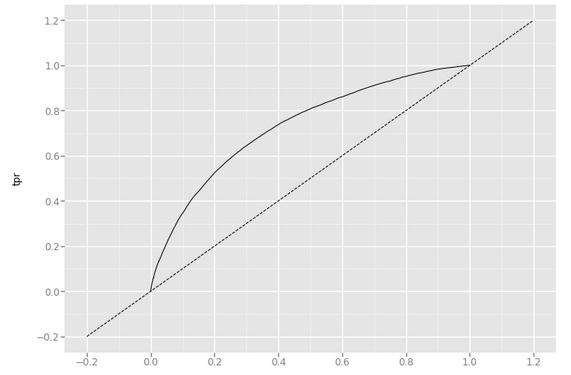
\includegraphics[width=5cm, keepaspectratio,]{fig010d.jpg}
	\caption{ROC curve showing 0.4 as the optimal threshold}
	\label{fig10d}
\end{figure} 

The results from the model are shown in figure \ref{fig10e}. We see that the recall and precision of play events (as denoted by 1) is very low suggesting that relying on a Bayesian approach centered around a weekly profile of each users habits is not an effective method for predicting a play event for a new time period.

\begin{figure}[h!]
	\centering
	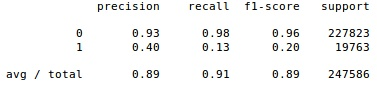
\includegraphics[width=7cm, keepaspectratio,]{fig010e.jpg}
	\caption{Beta-Bionmial Model Results}
	\label{fig10e}
\end{figure} 

\section{Feature analysis}

An advantage of logistic regression over non-linear models is that the coefficients are easily interpretable. While featuer engoneering was not the focus of this research an examination of these can yield insight into which features may be unecessary. 

\begin{figure}[h!]
	\centering
	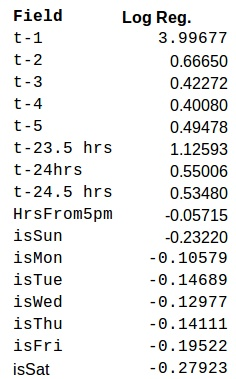
\includegraphics[width=4cm, keepaspectratio,]{fig014.jpg}
	\caption{}
	\label{fig14}
\end{figure} 

Fig \ref{fig14} shows that $t-1$ was by far the most important feature. This is expcted and it's importance crowds out the other features. Interestingly the t-24 hour period appears to have a stronger influence than $t-2$ to $t-5$ once $t-1$ has been accounted for. This reflects the daily patterns we observed in the preliminary analysis. The days of the week also pick up on the fact that weekeneds are somewhat different to weekdays thereby offering one area where the model could be simplified. Finally the hours from 5pm have a very small impact, and is likely unecessary if $t-24hrs$ is also used

\section{RNN Hyper parameter tuning}

For our evaluation of the RNN-LSTM model the dataset was reduced in order to perform the desired number of hyperparameter tests. It was found that the number of hidden layers, units, timeteps, samples, and iterations all played a signficant part in impacting the time it took to train the model. Typical run times were several hours long. 

Fig \ref{fig15} shows the results of some of the other tests that were performed. The improvment in performance comes with an increased in hidden layers, although this also leads to longer training times.

\begin{figure}[h!]
	\centering
	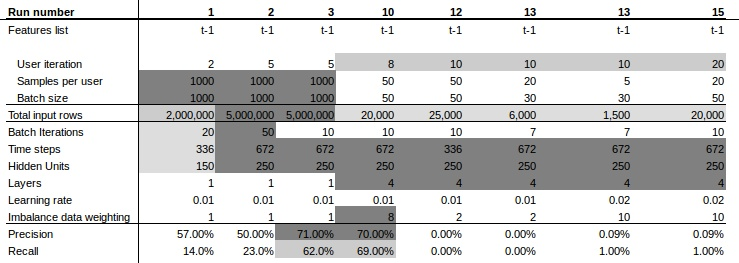
\includegraphics[width=7cm, keepaspectratio,]{fig015.jpg}
	\caption{}
	\label{fig15}
\end{figure}

\section{Adaptability to new users}

We also looked at the performance of models when it comes to learning the patterns of new users. Tie figures below show how the accuracy stablizied over time for each of the 10 test users. The periods indicate half-hourly intervals with 2-3,000 periods (1.5-2 months) appearing to be the time it takses to learn the habits of a typical user. 
\begin{figure}[h!]
	\centering
	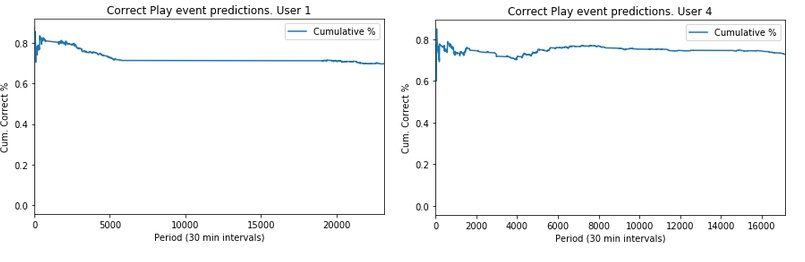
\includegraphics[width=7cm, keepaspectratio,]{fig008a.jpg}
	\caption{}
	\label{fig:fig8a}
\end{figure} 

\begin{figure}[h!]
	\centering
	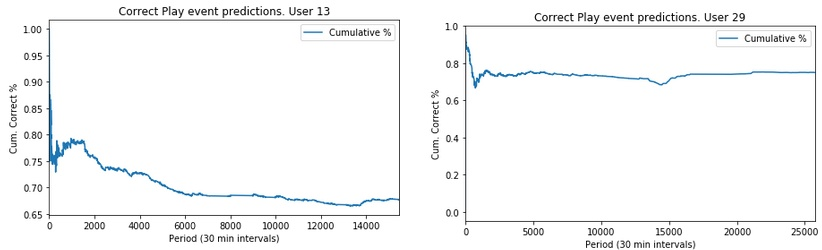
\includegraphics[width=7cm, keepaspectratio,]{fig008b.jpg}
	\caption{}
	\label{fig:fig8b}
\end{figure} 

\begin{figure}[h!]
	\centering
	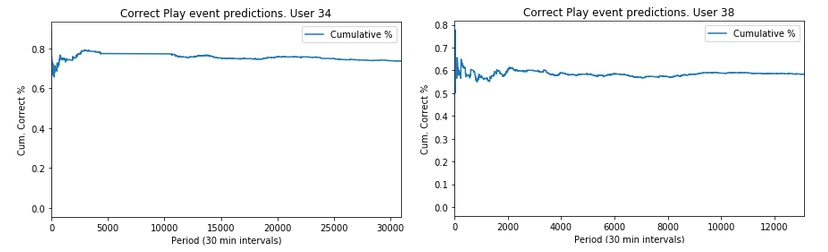
\includegraphics[width=7cm, keepaspectratio,]{fig008c.jpg}
	\caption{}
	\label{fig:fig8c}
\end{figure} 

\begin{figure}[h!]
	\centering
	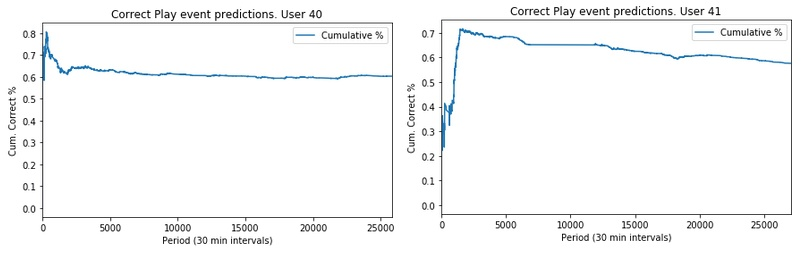
\includegraphics[width=7cm, keepaspectratio,]{fig008d.jpg}
	\caption{}
	\label{fig:fig8d}
\end{figure} 

\begin{figure}[h!]
	\centering
	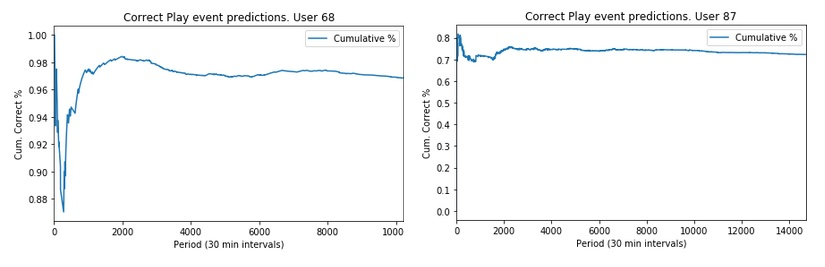
\includegraphics[width=7cm, keepaspectratio,]{fig008e.jpg}
	\caption{}
	\label{fig:fig8e}
\end{figure} 


From these charts it appears that two months worth of data is required to for the model to rget trained up on a new user.


\section{Content not used} % Main appendix title

Intro:
At an aggregate level, behaviour may appear to be deterministic, such as the times at which peak rush-hour occurs, but such behaviour is often composed of thousands or millions of individual stochastic processes such as the decisions made by individuals as to whether to leave work at 5pm or continue working a little longer.

While the modeling of aggregate patterns is well understood, these models ofen breakdown when applied to customizing results for individual users. At this level the temporal patterns of an individual combined with the behaviour of the population may be a better predictor of event timing. For instance, sticking with the example above, the times at which a person has lunch during the day may help predict that they will finish work a little later.


%\include{Appendices/AppendixB}
%\include{Appendices/AppendixC}

%----------------------------------------------------------------------------------------
%	BIBLIOGRAPHY
%----------------------------------------------------------------------------------------
\printbibliography[heading=bibintoc]

%----------------------------------------------------------------------------------------

\end{document}  
